\chapter{Systembeskrivelse}
Med udgangspunkt i projektformuleringen kommer dette projekts endelige system til at bestå af et software og hardware system, der kan tilsluttes et måleobjekt, hvorpå et blodtryk kan måles. Systemet skal kunne implementeres i forskningsmiljøer, hvor en eller flere forskere ønsker at analysere indhentede blodtrykssignaler. Visionen er, at systemet skal være let tilgængeligt og effektivt, hvilket vil komme til udtryk ved, at systemet fungerer stabilt.

I dette projekt realiseres en prototype af systemet. Det vil sige at flere dele af systemet udvikles ud fra forsimplede metoder i forhold til hvordan det vil være optimalt at implementere dem i virkeligheden. Her tænkes på hardware-, såvel som software-elementer. Hardwaren i prototypen realiseres på en printplade, således det er muligt at tage den med sig, samt er mere holdbar over tid. Softwaren i prototypen består af flere moduler. Disse er opbygget efter principperne i en trelagsmodel, hvilket vil sige, at koden indeholder et database-lag, logik-lag samt præsentation-lag. Dette er valgt for at skabe et overblik over hvilke dele af software-koden der har ansvaret for de enkelte funktionaliteter i systemet.

Hardwaren består af en forstærker og et filter. Forstærkeren opgave består i at forstærke det analoge signal fra max 11 millivolt til 5 volt. Filtret sørger for at filtrere unødig støj fra det analog signal. Signalændringen fra måleobjektet helt til visning af signal på graf er skitseret herunder. Det skal pointeres at dette kun er en skitse for at skabe overblik, derfor er flere processer i softwaren udeladt af diagrammet. 
\begin{figure}[htb]
	\centering
	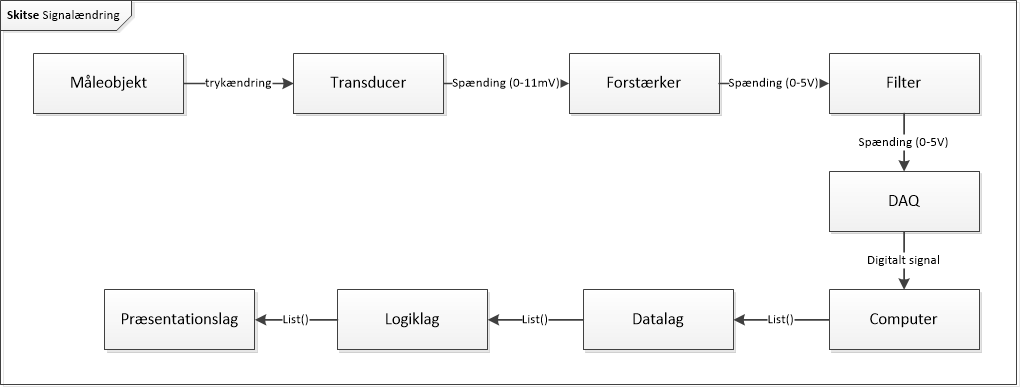
\includegraphics[width=1.0\textwidth]{Figurer/Signalandring}
	\caption{Skitse af signalændring}
	%\label{fig:Skitse der viser signalændring}
\end{figure}
Database-laget består af en lukket database samt indhentningen af blodtrykssignalet fra måleobjektet til transduceren gennem hardware inden det rammer software-delen. I den lukkede database gemmes det indhentede blodtrykssignal i en tabel. Signalet gemmes med et tidsstempel samt under et autogenereret nummer sammensat med det forsøgsnavn aktøren indtaster på brugergrænsefladen ved begyndelsen af en måling. \\
Logik-laget er handlingslaget, og alt kommunikation til de resterende lag går gennem dette lag. Laget indeholder flere klasser der indeholder metoder til indhentning af systoliske-, diastoliske og puls-værdier ud fra det indhentede blodtrykssignal. Derudover indeholder laget også klasser der har ansvaret for at foretage en filtrering af signalet når dette er valgt. \\ Præsentationslaget er aktørens vej ind i systemet, dette lag har til ansvar at udskrive valgte data på brugergrænsefladen. 

Systemet skal udadtil have en brugergrænseflade i form af en touch skærm eller almindelig computerskærm med tilhørende tastatur. Det er denne skærm som den primære aktører til systemet, altså forskeren, interagerer med. Det tilstræbes at opbygge brugergrænsefladen simpelt og efter forskerens logik, så opbygningen giver mening for systemets bruger. Efter indhentning af blodtrykssignal er systemet i stand til grafisk at vise signalet kontinuerligt, samt udskrive blodtrykssignalets systoliske-, diastoliske- og puls-værdier. Efter ønske kan systemets også alarmere, hvis signalet systoliske-værdier overskrider den definerede grænseværdien. Denne alarm vil være en indikation på at patienten, hvis blodtryk der vises kan lide af forhøjet blodtryk.
